\documentclass[a4paper,10pt]{article}

\usepackage[a4paper, total={6in, 9in}]{geometry}
\usepackage{graphicx}
\usepackage{svg}
\usepackage{mathtools}

\newlength\Colsep
\setlength\Colsep{10pt}

\usepackage{subfig}
\usepackage{amssymb}
\usepackage{amsfonts}
\usepackage{float}
\usepackage{amsmath}
\usepackage{caption}
\usepackage{subfig}
\usepackage{subfloat}
\usepackage{verbatim}
\usepackage{amsmath}


\usepackage[style=authoryear-comp, backend=biber]{biblatex}
\usepackage{fontspec}

\newcommand{\R}{\mathbb{R}}
\newcommand{\me}{\mathrm{e}}
\DeclareMathOperator{\EX}{\mathbb{E}}

\graphicspath{{./figures/}}

\begin{document}
\setlength\parindent{0pt}


\title{Assignment 1}
\clearpage\maketitle
\thispagestyle{empty}

\begin{abstract}

\end{abstract}

\newpage
\clearpage
\setcounter{page}{1}

\section{Introduction}
This assignment addresses three tasks in Machine Learning. First, two linear models are fit
to a simulated dataset and the expected relative performance is investigated. Furthermore,
the expected out of sample error, $E_{out}$, and the validation error $E_{val}$ for the best
model is calculated and compared. Secondly, the idea of regularization is introduced
when fitting a 10-th-order Legendre polynomial to a noisy sinusoidal. Moreover,
a 10-fold cross validation (CV) is performed in order to find the optimal value for the
regularization parameter, $\lambda$. Lastly, the topic of eigenfaces is examined. An eigenface is
a set of eigenvector used in computer vision problems of human face recognition.
Principal component analysis (PCA) is applied to a dataset of 400 images of human faces and
the eigenfaces is calculated. In addition, a random face is then reconstructed using the eigenfaces
obtained.

\section{Theory}
\subsection{Task 1}
It is considered a linear model given by
\begin{equation}
  y_i = 0.8x_i + \epsilon_i;\qquad -1 \leq x \leq1, i=1,...,N
  \label{eq:underlying_function}
\end{equation}
for the first problem. Here, $x$ $\sim$ Uniform(-1,1), $\epsilon_i$ $\sim$ Normal(0,1) and $N$ is the
size of the dataset. Furthermore, two linear models given by

\begin{alignat*}{2}
  g_1(x) = 0.5 + b_1x  &\qquad\text{and}\qquad g_2(x) = -0.5 + b_2x
\end{alignat*}
is fitted to the dataset. \newline

\subsection{Task 2}
For the second problem, the following model is considered
\begin{equation}
  y_i = \text{sin}(\pi x_i) + \epsilon_i;\qquad -1 \leq x \leq1, i=1,...,N
  \label{eq:sin}
\end{equation}
where $\epsilon_i$ $\sim$ Normal(0,1) and $N$ is the
size of the dataset. A model of the form
\begin{equation}
 y_i = \sum_{q=0}^{10} w_q L_q(x)
\end{equation}
is fitted to the model in Equation {\ref{eq:sin}}. Here, $L_q$ is a Legendre
polynomial of order $q$. Furthermore, the regularzer used is given by
\begin{equation}
  w = w^T w \leq C
\end{equation}
where C is some constant related to the regularization paramater $\lambda$.

\section{Method}
\subsection{Task 1}
A dataset of size $N\ = \ 30$ is simulated the the two models, $g_1$ and $g_2$, is fitted to
the dataset obtained from Equation {\ref{eq:underlying_function}}. In addition,
the expected slope of each model is calculated and the results can be seen in
Figure {\ref{fig:expected}}. \newline

In addition, 10,000 datasets of size $N\ =\ 30$ is simulated
by using model presented in Equation {\ref{eq:underlying_function}}. Each
dataset is split into a validation set of size $i$ and a training
set of size $30-i$ where $i = 5,...,25$. For every value of $i$, both models, $g_1$
$g_2$ is fitted to each of the training sets and the validation set is used
to choose the best model $g^*(x)$. Consequently, for each value of $i$
the expected errors for both $E_{out}(g^*)$ and $E_{val}(g^*)$. The two
expected errors are given by $E_{out}\ =\ \text{bias}^2 + noise$ and
$E_{val}$ is given by the mean squared residuals for the validation set. The results
can be seen in Figure {\ref{fig:noise}}.

\subsection{Task 2}
A 10-th order Legendre polynomial is fitted to the noisy sinusoidal in
Equation {\ref{eq:sin}} using regularisation parameter of
$\lambda\ =\ 0$ and $\lambda\ =\ 5$. Furthermore, the optimal
regularisation parameter is obtained using 10-fold cross-validation.

\subsection{Task 3}
The \texttt{pixmap}-package in \texttt{R} is used to read the images. Furthermore, the
\texttt{prcomp} from the \texttt{stats}-package is used to perform
the principal component analysis. Consequently, a face number 115 is
reconstructed using the first 5, 50 and 200 eigenfaces.

\section{Results}
\subsection{Task 1}
Two models, $g_1$ and $g_2$ is fitted to a noisy dataset of size $N\ =\ 30$. The expected
both models averaged over 10,000 runs is seen in Figure {\ref{fig:expected}} and it is seen
that the two models are expected to perform equally well in the long run. Moreover, it is observed
in Figure {\ref{fig:noise}} both models is seen alongside with the noisy dataset as well
as the true underlying function. \newline

The expected errors for both $E_{out}$ and $E_{val}$ is visualized in Figure {\ref{fig:e_val_e_out}}.
It can be observed that $E_{val}$ always gives an underestimated value for
the out of sample error.

\begin{figure}[H]
  \subfloat[][The expected slope for model $g_1$ and $g_2$ \\averaged over 10,000 runs.]{
  \def\svgwidth{0.48\linewidth}
  {\input{figures/expected.ps_tex}}
  \label{fig:expected}}
  \subfloat[][Model $g_1$ and $g_2$ plottet together with \\Equation {\ref{eq:underlying_function}} and the true underlying
   function $y = 0.8x$]{
  \def\svgwidth{0.48\linewidth}
  {\input{figures/task1i.ps_tex}}
  \label{fig:noise}} \\
  \centering
  \subfloat[][$E_{out}$ and $E_{val}$]{
  \def\svgwidth{0.48\linewidth}
  {\input{figures/task1ii.ps_tex}}
  \label{fig:e_val_e_out}}
  \caption{In \protect \subref{fig:expected} the average slope of $g_1$ and $g_2$ is plotted and in \protect \subref{fig:noise}
  the two models are fitted to the model in Equation {\ref{eq:underlying_function}}. In \protect \subref{fig:e_val_e_out} $E_{val}$ and $E_{out}$is seen. }
\end{figure}

\subsection{Task 2}
For the fitting problem in Task 2, a 10th-order Legendre polynomial is cosidered to
fit the target function.
\begin{figure}[H]
  \subfloat[][The noisy sinusoidal and the true underlying\\ function from Model {\ref{eq:sin}}]{
  \def\svgwidth{0.48\linewidth}
  {\input{figures/sin_y.ps_tex}}
  \label{fig:sin_noise}}
  \subfloat[][Two regularized models with $\lambda = 0$ and $\lambda = 5$ is plotted.]{
  \def\svgwidth{0.48\linewidth}
  {\input{figures/task2i.ps_tex}}
  \label{fig:reg_5_2}} \\
  \subfloat[][It is seen the CV-error for the fitted model as a\\
  function of increasing $\lambda$]{
  \def\svgwidth{0.48\linewidth}
  {\input{figures/cv.ps_tex}}
  \label{fig:cv}}
  \subfloat[][The best regularized model is seen having $\lambda = 2.7$]{
  \def\svgwidth{0.48\linewidth}
  {\input{figures/best.ps_tex}}
  \label{fig:best}}

  \caption{It is seen in \protect \subref{fig:sin_noise} the noisy and the underlying function
  of Model {\ref{eq:sin}} and it is visualised the impact of regularization in
  \protect \subref{fig:reg_5_2} and
  in \protect \subref{fig:cv} it is seen the
  CV-error for the fitted model with increasing $\lambda$. In \protect
  \subref{fig:best} the best regularized model is seen.
  }
\end{figure}

\subsection{Task 3}
\begin{figure}[H]
  \subfloat[][The mean image]{
    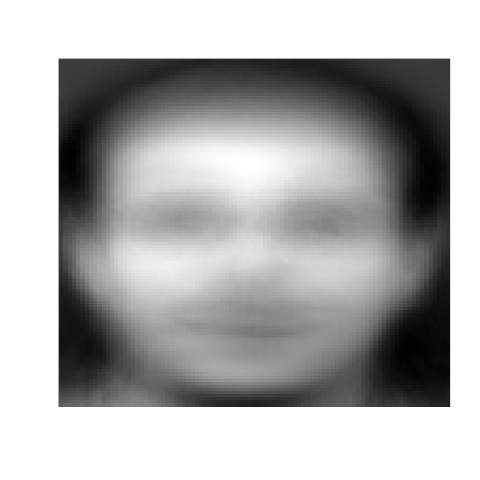
\includegraphics[width=0.5\linewidth]{mean_face.png}
    \label{fig:mean_face}
  }
  \subfloat[][Standard Deviation image]{
    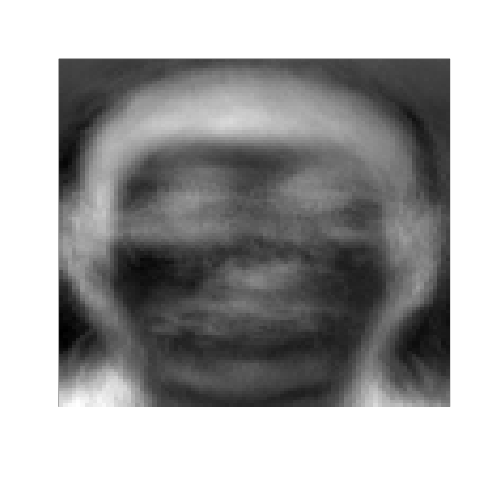
\includegraphics[width=0.5\linewidth]{sd_face.png}
    \label{fig:sd_face}
  } \\
  \subfloat[][Original version of image 168]{
    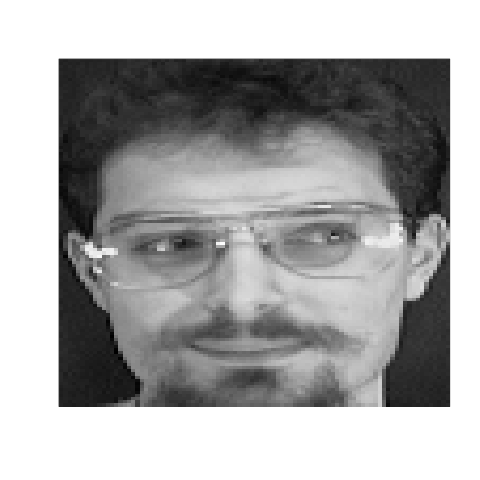
\includegraphics[width=0.5\linewidth]{original_face.png}
    \label{fig:original}
  }
  \subfloat[][Scaled version of image 168]{
    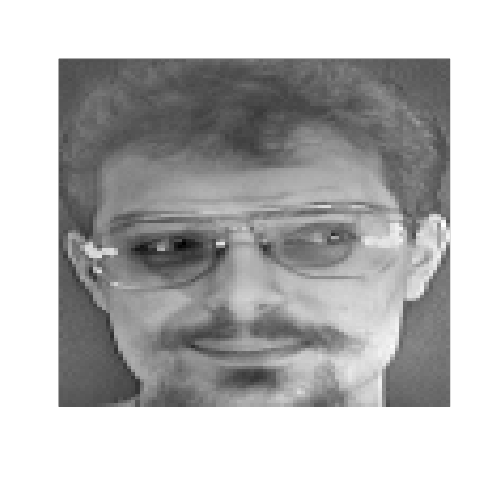
\includegraphics[width=0.5\linewidth]{scaled_face.png}
    \label{fig:scaled}
  }

  \caption{Eigenface}
\end{figure}

two is fitted to a random 10th-order target function and the relative performance of the two is compared using a measure of overfitting.
Secondly, a sequence of random target functions of higher order is generated and the
relative performance between the two hypothesis is again compared for different combinations of
datasets of different sizes and target functions of different orders

\begin{figure}[H]
  \subfloat[][First eigenface]{
    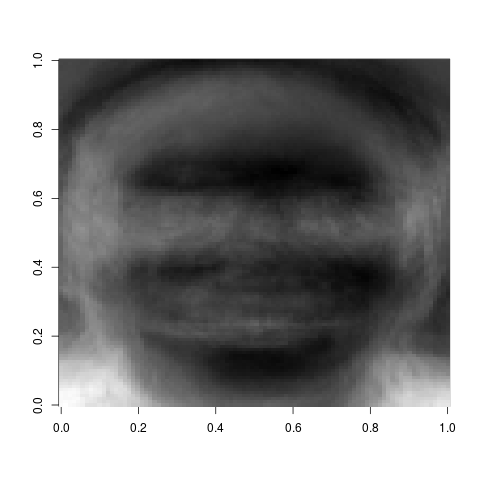
\includegraphics[width=0.20\linewidth]{eigen_1.png}
    \label{fig:mean_face}
  }
  \subfloat[][Second eigenface]{
    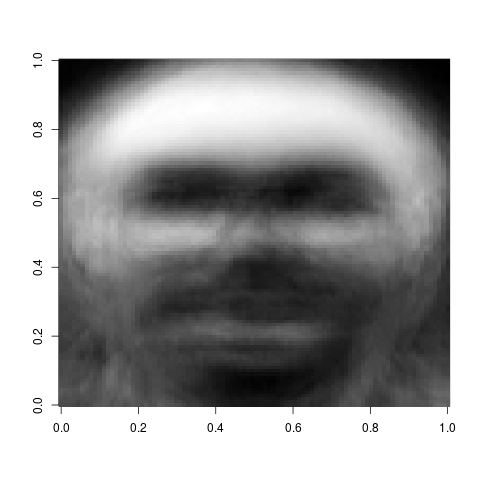
\includegraphics[width=0.20\linewidth]{eigen_2.png}
    \label{fig:sd_face}
  }
  \subfloat[][Third eigenface]{
    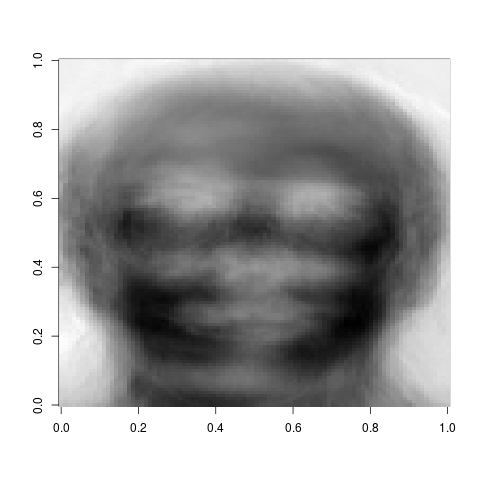
\includegraphics[width=0.20\linewidth]{eigen_3.png}
    \label{fig:original}
  }
  \subfloat[][Fourth eigenface]{
    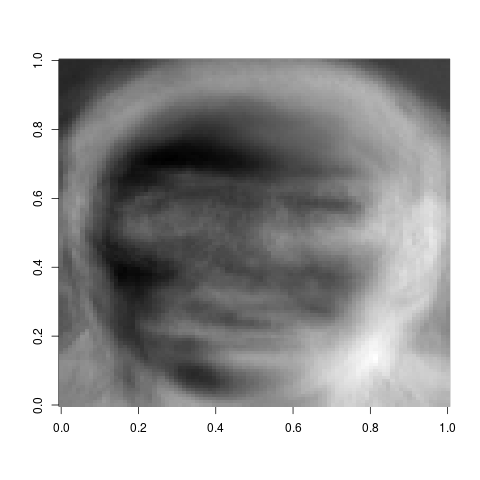
\includegraphics[width=0.20\linewidth]{eigen_4.png}
    \label{fig:scaled}
    }
  \subfloat[][Fifth eigenface]{
    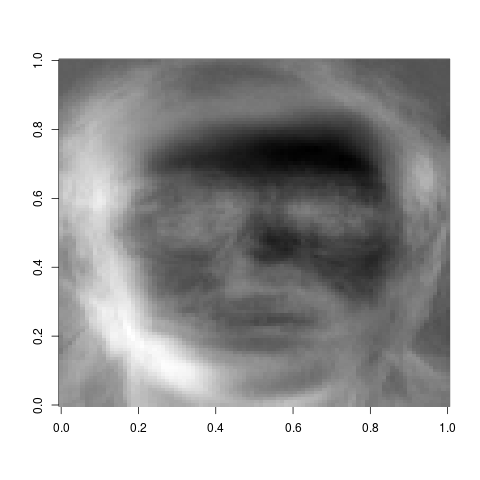
\includegraphics[width=0.20\linewidth]{eigen_5.png}
    \label{fig:scaled}
  } \\
  \subfloat[][Sixth eigenface]{
    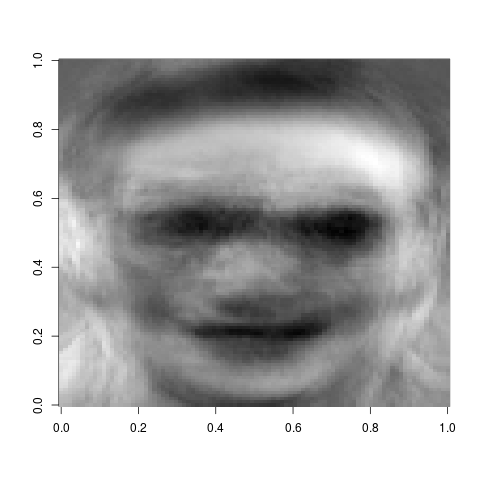
\includegraphics[width=0.20\linewidth]{eigen_6.png}
    \label{fig:mean_face}
  }
  \subfloat[][Seventh eigenface]{
    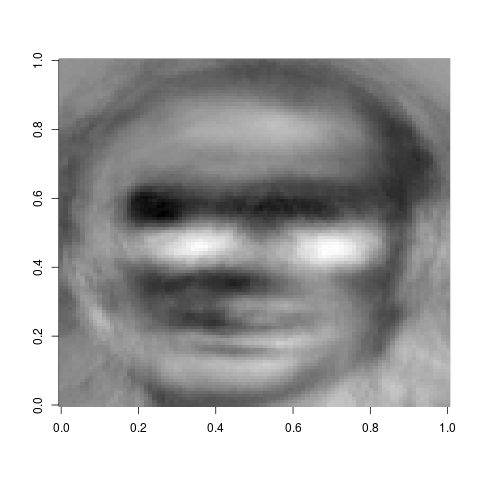
\includegraphics[width=0.20\linewidth]{eigen_7.png}
    \label{fig:sd_face}
  }
  \subfloat[][Eigth eigenface]{
    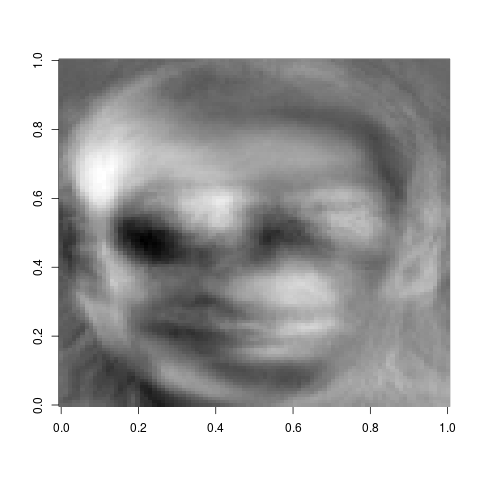
\includegraphics[width=0.20\linewidth]{eigen_8.png}
    \label{fig:original}
  }
  \subfloat[][Ninth eigenface]{
    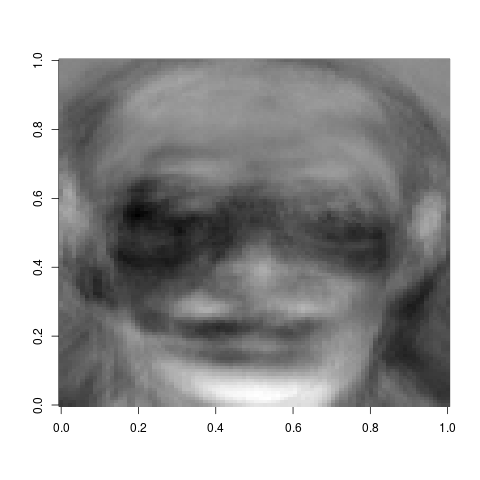
\includegraphics[width=0.20\linewidth]{eigen_9.png}
    \label{fig:scaled}
    }
  \subfloat[][Tenth eigenface]{
    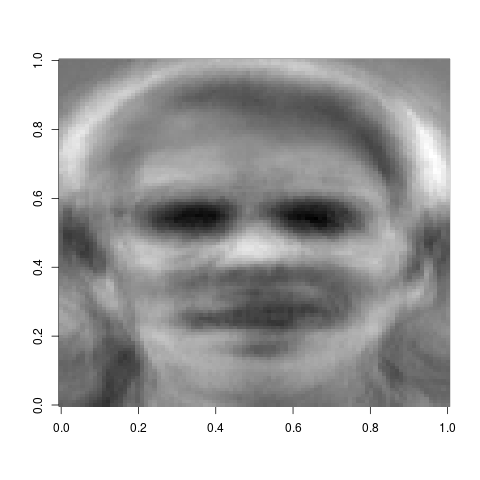
\includegraphics[width=0.20\linewidth]{eigen_10.png}
    \label{fig:scaled}
  }
  \caption{Eigenface}
\end{figure}

two is fitted to a random 10th-order target function and the relative performance of the two is compared using a measure of overfitting.
Secondly, a sequence of random target functions of higher order is generated and the
relative performance between the two hypothesis is again compared for different combinations of
datasets of different sizes and target functions of different orders


\begin{figure}[H]
  \subfloat[][First eigenface]{
    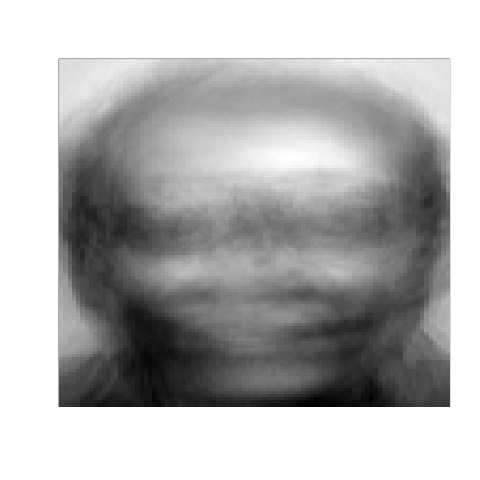
\includegraphics[width=0.5\linewidth]{recon_5_eigenfaces.png}
    \label{fig:mean_face}
  }
  \subfloat[][Second eigenface]{
    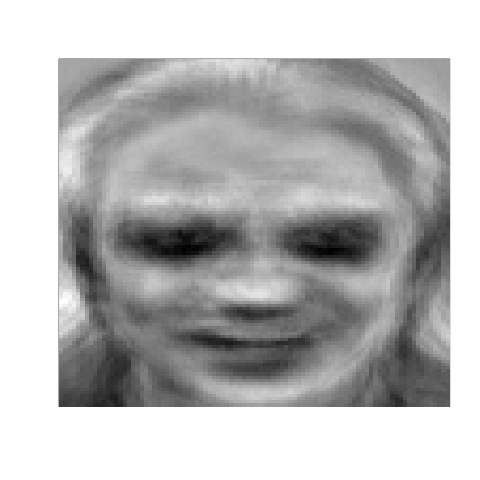
\includegraphics[width=0.5\linewidth]{recon_50_eigenfaces.png}
    \label{fig:sd_face}
  } \\
  \subfloat[][Tenth eigenface]{
    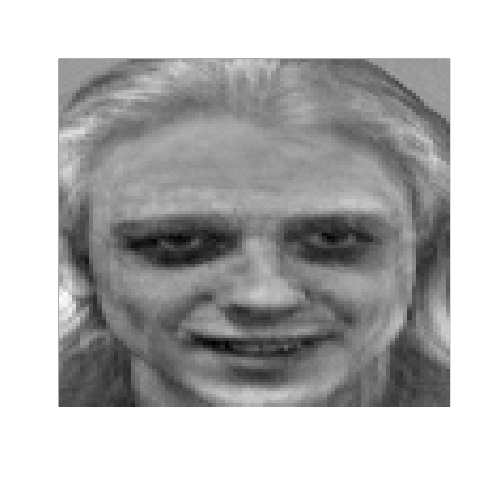
\includegraphics[width=0.5\linewidth]{recon_200_eigenfaces.png}
    \label{fig:scaled}
  }
  \subfloat[][Tenth eigenface]{
  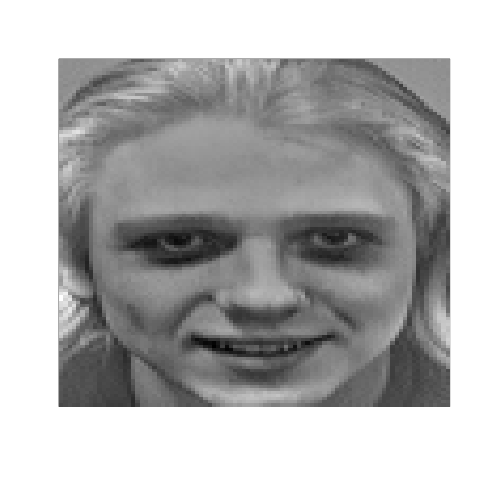
\includegraphics[width=0.5\linewidth]{scaled_115.png}
  \label{fig:scaled}
  }
  \caption{Eigenface}
\end{figure}


\section{Appendix}


\begin{verbatim}



\end{verbatim}


\end{document}
